%%%%%%%%%%%%%%%%%%%%%%%%%%%%%%%%%%%%%%%%%%%%%%%%%%%%%%%%%%%%%%%%%%%%%%%%%%%
%                                                                         %
%  KES 2002 (Crema, Italy)                                                %
%    Missing Value Estimation by Local Minor Components                   %
%    Chi-Hyon Oh, Katsuhiro Honda and Hidetomo Ichihashi                  %
%                                                                         %
%%%%%%%%%%%%%%%%%%%%%%%%%%%%%%%%%%%%%%%%%%%%%%%%%%%%%%%%%%%%%%%%%%%%%%%%%%%

%\documentstyle[epsbox,12pt]{ioscrcb}
\documentclass{article}
\usepackage{graphicx}
\addtolength{\oddsidemargin}{-15mm}  %
\addtolength{\evensidemargin}{-15mm}  %
\setlength{\textheight}{210mm}    %
\setlength{\textwidth}{150mm}     %


\newcommand{\vctr}[1]{\mbox{\boldmath $#1$}}

\begin{document}

\title{Missing Value Estimation by \\ Local Minor Components}

\author{Chi-Hyon Oh${}^\dagger$, Katsuhiro Honda${}^\ddagger$, and Hidetomo Ichihashi${}^\ddagger$\\${}^\dagger$ Faculty of Liberal Arts and Sciences, Osaka University of Economics and Law,\\
6-10 Gakuonji, Yao, Osaka, 581-8511 Japan\\
${}^\ddagger$ Graduate School of Engineering, Osaka Prefecture University,\\
1-1 Gakuen-cho, Sakai, Osaka, 599-8531 Japan\\ 
}

\date{}

\maketitle
\pagestyle{plain}
\pagestyle{plain}
\thispagestyle{plain}

%%%%%%%%%%%%%%%%%%%%%%%%%%%%%%%%%%%%%%%%%%%%
%                Abstract                  %
%%%%%%%%%%%%%%%%%%%%%%%%%%%%%%%%%%%%%%%%%%%%

\begin{abstract}
In this paper, we propose a method of estimating missing values by local minor components. We assume that a data point, some attributes of which are missing, is on a hyper plane. The normal of the hyper plane is a local minor component vector. Thus, the data point is projected onto the hyper plane and its missing attributes are estimated. We extract the local minor components by executing fuzzy clustering and neural principal component analysis (PCA) approach simultaneously. The extracted local minor components take the substructures of the data set into consideration. Missing values are estimated simply and easily.
\end{abstract}

%%%%%%%%%%%%%%%%%%%%%%%%%%%%%%%%%%%%%%%%%%%%
%                Introduction              %
%%%%%%%%%%%%%%%%%%%%%%%%%%%%%%%%%%%%%%%%%%%%

\section{Introduction} 
%
Generally, principal components are extracted as eigen vectors associated with larger eigen values of a covariance matrix of a given data set. Oja \cite{Oja1} has proposed a technique of extracting principal components by neural networks which conduct Hebbian learning instead of the eigen value problem. He also has shown that the neural PCA approach can be applied for extracting minor components \cite{Oja2}.

In this paper, we propose a method of estimating missing values by local minor components. To extract the local minor components, we employ the neural PCA approach and implement the fuzzy clustering \cite{Hoppner} at the same time. Partitioning the data set into some clusters enables us to take its substructures into consideration. The local minor components well represent the distinctive structures of the data set. Hence, we can expect our method can achieve good missing value estimation by using the extracted local minor components. In the numerical example, we apply our method to a three dimensional artificial data set and examine its performance.

%%%%%%%%%%%%%%%%%%%%%%%%%%%%%%%%%%%%%%%%
% Extraction of Local Minor Components %
%%%%%%%%%%%%%%%%%%%%%%%%%%%%%%%%%%%%%%%%

\section{Extraction of Local Minor Coponents}
%
Fuzzy $c$-Varieties (FCV) \cite{Bezdek} proposed by Bezdek forms fuzzy clusters by minimizing the sum of distances from data points to prototypes.  The prototypes of the FCV are multi dimensional linear varieties spanned by some vectors. We denote a data point and a vector spanning the prototypes as follows:
%
\begin{eqnarray}
	{\vctr x}_i=(x_{i1},\cdots,x_{iK})^{\top}, \qquad i=1,\cdots,N.
\end{eqnarray}
%
\begin{eqnarray}
	{\vctr w}_{ck}=(w_{ck1},\cdots,w_{ckK})^{\top}, \qquad c=1,\cdots,C, \ k=1,\cdots,K-m.
\end{eqnarray}
%
where $N$ and $C$ represents the number of data points and that of clusters respectively. $K$ is the dimensionality of the data points and $m$ is the number of minor component vectors. If we regard ${\vctr w}_{ck}$ as the principal component vector, the FCV can be said to be the simultaneous analysis of the fuzzy clustering and the PCA.

Let us consider minor components now. The clustering criterion of the FCV can be written as follows by the minor component vectors.
%
\begin{eqnarray}
	\sum_{c=1}^{C} \sum_{i=1}^{N} \sum_{k=K-m+1}^{K} u_{ci}{\vctr w}_{ck} ^{\top} ({\vctr x}_i - {\vctr v}_c )  ({\vctr x}_i - {\vctr v}_c ) ^{\top}  {\vctr w}_{ck}.
	\label{eq:criterion}
\end{eqnarray}
%
Note that ${\vctr w}_{ck}$ in (\ref{eq:criterion}) represents the minor component vector and ${\vctr v}_c$ does the cluster center of the cluster $c$. $u_{ci}$ is membership of the data point to the cluster which represents degree of belonging to the cluster. $u_{ci}$ satisfies the following condition. 
%
\begin{eqnarray}
{\vctr u}_c \in \{ (u_{ci}) | \sum_{c=1}^C u_{ci}= 1, u_{ci} \in [ 0,1 ], 
c = 1, \cdots , C \}.
\label{eq:mem}
\end{eqnarray}
%

Optimization of (\ref{eq:criterion}) is resolved into minimization of the following objective function $L$ according to Lagrange's method of indeterminate multiplier.

%
\begin{eqnarray}
L &=& \sum_{c=1}^{C} \sum_{i=1}^{N} \sum_{k=K-m+1}^{K} u_{ci} {\vctr w}_{ck} ^{\top} ({\vctr x}_i - {\vctr v}_c )  ({\vctr x}_i - {\vctr v}_c ) ^{\top}  {\vctr w}_{ck} \nonumber \\
&+& T_0 \sum_{c=1}^{C} \sum_{i=1}^{N} u_{ci} \log u_{ci} + \sum_{i=1}^{N} T_i \biggl( \sum_{c=1}^{C} u_{ci} -1 \biggr).
\label{eq:objective}
\end{eqnarray}
%
In (\ref{eq:objective}), the first term represents the clustering criterion of the FCV. The second term represents entropy maximization as regularization which was introduced in Fuzzy $c$-Means (FCM) by Miyamoto {\it et al.} \cite{Miyamoto}. It enables us to obtain fuzzy clusters. The FCM is the most popular fuzzy clustering algorithms. $T_0>0$ is the weighting parameter which specifies degree of fuzziness. The remaining terms describe the constraint of the membership $u_{ci}$, {\it i.e.} (\ref{eq:mem}). $T_i$ is the Lagrangian multiplier.

From the necessary condition $ {\partial L}/{\partial v_{ck}} = 0$ and ${\partial L}/{\partial u_{ci}} = 0$ for the optimality of the objective function $L$, we can calculate cluster centers and memberships as follows:
%
\begin{eqnarray}
	v_{ck} = \sum_{i=1}^N u_{ci} \ \Big/ \ x_{ik}\sum_{i=1}^N u_{ci}.
\label{eq:v}
\end{eqnarray}
%
\begin{eqnarray}
	u_{ci} &=& \exp A_{ci} \ \Big/ \ \sum_{l=1}^{C} \exp A_{li}.
\label{eq:u}
\end{eqnarray}
%
where�C
%
\begin{eqnarray}
A_{li} &=& -\frac{1}{T_0} \sum_{k=K-m+1}^{K}{\vctr w}_{lk} ^{\top} ({\vctr x}_i - {\vctr v}_l ) ({\vctr x}_i - {\vctr v}_l ) ^{\top} {\vctr w}_{lk}.
\end{eqnarray}
%

We extract the local minor component vectors by the neural PCA approach. From the necessary condition $\partial{J} / \partial{\vctr w_{ck}}$, we have the following equation.
%
\begin{eqnarray}
	\frac{\partial{J}}{\partial{\vctr w_{ck}}} = 2 \sum_{i=1}^{N} u_{ci} ({\vctr x}_i - {\vctr v}_c ) ({\vctr x}_i - {\vctr v}_c ) ^{\top}  {\vctr w}_{ck}.
	\label{eq:dif_minor}
\end{eqnarray}
%
Taking normalization and orthogonalization into account, we could derive the following learning rule to extract the local minor component vectors.
%
\begin{eqnarray}
	\Delta {\vctr w}_{ck} &=& \gamma u_{ci} 
	\bigg\{-{y}_{ck}({\vctr x}_i- {\vctr v}_c ) \nonumber \\
	&+& \Bigl({y}_{ck}^2 +1 -({\vctr w}_{ck}^{old})^{\top} {\vctr w}_{ck}^{old}\Bigl){\vctr w}_{ck}^{old} - \alpha\sum_{l>k}{y}_{cl}{y}_{ck} {\vctr w}_{cl}^{old}\bigg\}.
	\label{eq:w}
\end{eqnarray}
where $\gamma>0$ denotes the learning rate and $\alpha>0$ does the coefficient of the orthogonalization. If $\alpha$ is sufficiently large, each local minor component vector is supposed to be orthogonalized.

The solution algorithms for our method are based on an iterative procedure. We remark them below.
\\ \\
\noindent
{\it Extracting Algorithms of the Local Minor Components}

\noindent
Step 1: Set each parameter and the terminal condition $\epsilon > 0$. Initialize memberships. \\
Step 2: Update cluster centers by using (\ref{eq:v}).\\
Step 3: Extract local minor components by using (\ref{eq:w}).\\
Step 4: Update memberships by using (\ref{eq:u}).\\
Step 5: If $\max | u_{ck}^{NEW} - u_{ck}^{OLD} | < \epsilon $, then stop. Otherwise, return to Step 2.
\\
%
%%%%%%%%%%%%%%%%%%%%%%%%%%%%%%%%%%%%%%%%%%%%%%%%%%%%%%
% Missing Value Estimation by Local Minor Components %
%%%%%%%%%%%%%%%%%%%%%%%%%%%%%%%%%%%%%%%%%%%%%%%%%%%%%%

\section{Missing Value Estimation by Local Minor Components}
%
We exploit the extracted local minor components by the pre-mentioned algorithms to estimate the missing values. We assume that a data point some attributes of which are missing is on a hyper plane. The normal of the hyper plane is a local minor component vector. Thus, the data point is projected onto the hyper plane and its missing attributes are estimated. To begin with, the data points are decided which hyper plane they are to be projected onto since the data set is fuzzily partitioned. In this study, we employ the maximum membership rule which has the data points belong to the cluster with the maximum membership.

Suppose an attribute ${x}_{il}$ is missing in the data points ${\vctr x}_i$. To estimate ${x}_{il}$, we consider a $K-1$ dimensional hyper plane whose normal is a local minor component vector ${\vctr w}_{cK}$. The linear equation for the hyper plane can be written as follows:
%
\begin{eqnarray}
	({\vctr x}_i - {\vctr v}_c )^T {\vctr w}_{cK} = 0.
	\label{eq:xw0}
\end{eqnarray}
%
If it is assumed that ${x}_{il}$ is on the hyper plane. From (\ref{eq:xw0}), we can derive it by the following equation.
%
\begin{eqnarray}
	{x}_{il} = -\frac{1}{{w}_{cl}} \sum_{m=1,m\not= l}^{M} ({x}_{im} - {v}_{cm}) 
	{w}_{cm}+{v}_{cl}.
	\label{eq:repair}
\end{eqnarray}
%
If two attributes are missing, another hyper plane whose normal is the second minor component vector ${\vctr w}_{cK-1}$ is derived.
%
\begin{eqnarray}
	({\vctr x}_i - {\vctr v}_c )^T {\vctr w}_{cK-1} = 0
	\label{eq:xw20}
\end{eqnarray}
%
From (\ref{eq:xw0}) and (\ref{eq:xw20}), we can estimate two missing attributes. Thus, we can estimate any numbers of missing attributes if the same numbers of minor component vectors are extracted.

%%%%%%%%%%%%%%%%%%%%%
% Numerical Example %
%%%%%%%%%%%%%%%%%%%%%

\section{Numerical Example}
%
In the numerical example, we apply our method to a three dimensional artificial data set and estimate the missing values. Figure \ref{fig:3Ddata} shows the data set used in the numerical example. The data set consists of 20 data points and two out of them are missing one attribute. Besides, the data set has a data point where two attributes are missing. From Figure \ref{fig:3Ddata}, we can notice that the data set has two substructures, the upper part and lower one. The following parameters are employed.
%
%%%%%%%%%%% figure 6 %%%%%%%%%%%%%%%%%%%
\begin{figure}[t]
	\begin{center}
		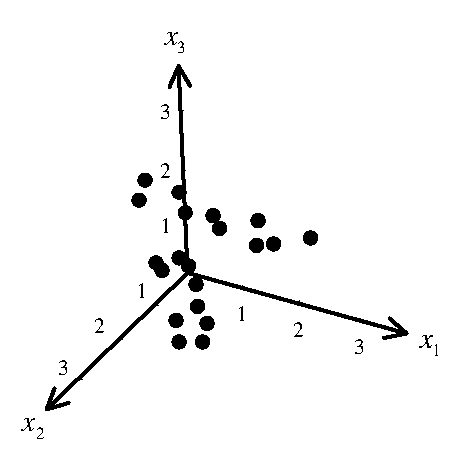
\includegraphics[height=60mm,clip]{3D.eps} 
		\caption{The three dimensional artificial data set.}
		\label{fig:3Ddata}
	\end{center}
\end{figure}
%%%%%%%%%%%%%% End %%%%%%%%%%%%%%%%%%%%
%
\begin{quotation}
\noindent
The number of clusters $C$: 2\\
Entropy coefficient $T_{0}$: 0.2\\
Learning rate for the Hebbian learning $\gamma$: 0.000001\\
Coefficient of orthogonalization $\alpha$: 10\\
The terminal condition of iterative procedure $\varepsilon$: 0.001 \\
\end{quotation}

The results of missing value estimation plotted on the two dimensional diagrams are shown in Figure 2 (a) and (b). The exact values by the estimations are also shown in Table 1. The estimated attributes are written in the bold numbers in Table 1. In Figure 2 (a) and (b), ��s represent the cluster center ${\vctr v}_{c}$. �Zs and ��s depict the data points belonging to the two different clusters respectively. As we mentioned in the previous section, we have the data points belong to the cluster with the maximum membership. �~s are data points with missing attributes. The data points connected with �~s by the dotted lines are the estimated ones by our method. From Figure 2 (a), (b) and Table 1, we can see that good missing value estimation considering substructures of the data set is achieved.

%%%%%%%%%%%%%%%%%%%%%%%%%%%%%%%
%%  Figure data
%%%%%%%%%%%%%%%%%%%%%%%%%%%%%%%
\begin{figure}[tb]
	\begin{center}
		\hspace{-4mm}
		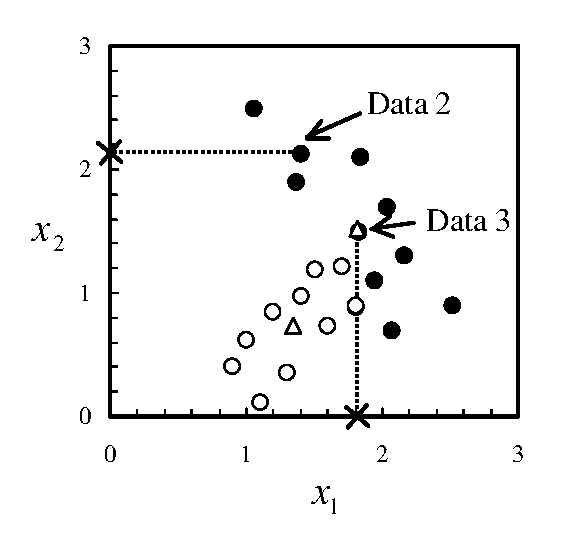
\includegraphics[height=60mm,clip]{3dim12.eps} 
		\hspace{10mm}
		\includegraphics[height=60mm,clip]{3dim23.eps}\\ 
		\hspace{5mm}(a) $x_1-x_2$ plane.\hspace{45mm}(b) $x_2-x_3$ plane.
		\vspace{-1mm}
		\caption{The results of missing value estimation.}
		\vspace{-8mm}
		\label{fig:data}
	\end{center}
\end{figure}
%

%%%%%%%%%%%%%%
% Conclusion %
%%%%%%%%%%%%%%
%
\section{Conclusion}
%
In this paper, we have proposed a method estimating missing values by local minor components. We extracted the local minor components by executing the fuzzy clustering and the neural PCA approach simultaneously. In the numerical example, we applied our method to a three dimensional artificial data set and estimated its missing values. The results showed the good missing value estimation considering substructures of the data set has been done by our method.

%%%%%%%%%%% table 1 %%%%%%%%%%%%%%%%%%%
\begin{table}[t]
	\caption{The results of missing value estimation.}
	\label{table23}
	\begin{center}
		\begin{tabular}{|c|c|c|c|} \hline
			 & ${x}_{1}$ & ${x}_{2}$ & ${x}_{3}$ \\ \hline
			Data1	& 1.30  & 0.36 & {\bf 0.97} \\ \hline
			Data2	& 1.40 & {\bf 2.12} & 2.02  \\ \hline
			Data3	& {\bf 1.82}  & 1.50 & {\bf 2.51} \\ \hline
		\end{tabular}
	\end{center}
\end{table}
%%%%%%%%%%%%%% End %%%%%%%%%%%%%%%%%%%%


%%%%%%%%%%%%%%%%%%%%%%%%%%%%%%
%         Bibliography       %
%%%%%%%%%%%%%%%%%%%%%%%%%%%%%%

\begin{thebibliography}{99}

\bibitem{Oja1}
E.Oja, A Simplified Neuron Model as a Principal Component Analyzer, Journal of Mathematical Biology 15 (1982) 267-273.

\bibitem{Oja2}
E.Oja, Principal Components, Minor Components, and Linear Neural Networks, Neural Networks 5 (1992) 195-204.

\bibitem{Hoppner}
F. H\"{o}ppner, F. Klawonn, R. Kruse and T. Runkler, {\it Fuzzy cluster analysis}, John Wiley \& Sons, Chichester (1999).

\bibitem{Bezdek}
J.C.Bezdek, C.Coray, R.Gunderson and J.Watson, Detection and Characterization of Cluster Substructure 2. Fuzzy $c$-Varieties and Convex Combinations Thereof, SIAM J. Appl. Math. 40, 2 (1981) 358-372.

\bibitem{Miyamoto}
S. Miyamoto and M. Mukaidono, Fuzzy $c$-Means as a Regularization and Maximum Entropy Approach, Proc. IFSA'97 2 (1997) 86-92.

\end{thebibliography}

\end{document}
